\section{Wykład 7 - sieci RBF (Radial Basis Functions)}

\begin{figure}[H]
 \centering
 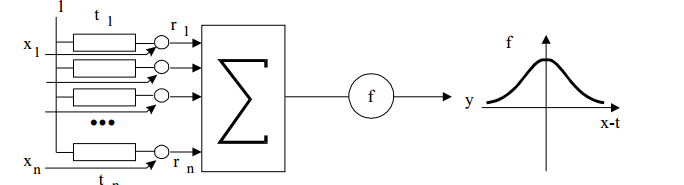
\includegraphics[scale=0.6]{radial}
\end{figure}

Neuron radialny - Agregacja sygnałów wejściowych
w tym typie neuronu polega na 
obliczaniu odległości pomiędzy 
obecnym wektorem wejściowym X
a ustalonym podczas uczenia 
centroidem pewnego podzbioru T.

Również nieliniowa funkcja 
przejścia w tych neuronach ma 
odmienną formę - „dzwonu” 
gaussoidy - czyli jest funkcją
niemonotoniczną.

Sieć typu RBF 
w zastosowaniu 
do klasyfikacji 
(wykrywa
i sygnalizuje 
skupiska 
danych 
wejściowych)

\paragraph{Neuron radialny} jest zdefiniowany przez swoje centrum i parametr - promień.
Obliczana jest odległość wektora wag i wektora sygnałów. Promień jest przechowywany
w neuronie jako wartość progowa.

\paragraph{Powtórne próbkowanie} Metoda ta polega na tym, że wybrane w sposób 
losowy elementy ze zbioru uczącego kopiowane są do neuronów radialnych 
(jako występujące w tych neuronach zestawy wag). Ponieważ podlegające 
kopiowaniu sygnały wejściowe wybrane zostały w sposób losowy, więc 
"reprezentują" one (w sensie statystycznym) rozkład wszystkich danych 
uczących. Jednakże, jeśli liczba neuronów radialnych nie jest duża, to neurony 
te mogą stanowić w rzeczywistości złą reprezentację (Haykin, 1994).

\paragraph{ k-średnich} Algorytm ten (Bishop, 1995) próbuje ustalić optymalny 
zbiór punktów, które stanowić będą centra skupień występujących w danych 
uczących. Mając K neuronów radialnych musimy wytworzyć K niezależnych 
centrów, w taki sposób, by reprezentowały one charakterystyczne skupiska 
wejściowych danych. Centra te ustala się w procesie iteracyjnym, w którym 
powtarzane są następujące czynności
\begin{enumerate}
 \item Każdy element zbioru uczącego przypisywany jest do tego centrum 
skupienia, które położone jest bliżej danego elementu niż wszystkie pozostałe 
centra
 \item Każde centrum skupienia wyznaczane jest jako wektor średnich wartości 
zmiennych wyznaczony dla wszystkich punktów należących do danego 
skupienia
\end{enumerate}
 
 \paragraph{Wybór promienia (odchylenia)}
 
 Definiowanie przez użytkownika. Użytkownik samodzielnie określa wielkość
odchylenia.
Równomierny przydział odchyleń. Odchylenie (identyczne dla wszystkich 
neuronów) jest określane za pomocą pewnej reguły heurystycznej, 
uwzględniającej liczbę centrów oraz wielkość zajmowanej przez nie 
przestrzeni (Haykin, 1994).
Przydział metodą k-najbliższych sąsiadów. Odchylenie dla każdego 
neuronu jest określane indywidualnie jako średnia odległość do jego k 
najbliższych sąsiadów (przypadków ze zbioru danych). Stąd odchylenia są
mniejsze w mocno zagęszczonym obszarze danych, co umożliwia zachowanie 
drobnych szczegółów i większe w obszarze, w którym dane występują rzadko 
(umożliwia to lepszą interpolację).

Zastosowanie RBF (zamiast MLP) 
spowoduje, że sieć neuronowa znajdzie 
aproksymację lepiej dopasowaną do 
lokalnych właściwości zbioru danych, 
ale gorzej ekstrapolującą.
\textbf{Sieci RBF bywają nadmiernie wrażliwe 
na nawet nieliczne błędy w danych 
uczących}

\paragraph{Sieć RBF} Ma ona strukturę dwuwarstwową, warstwa ukryta realizuje odwzorowanie 
nieliniowe realizowane przez neurony radialnej funkcji bazowej. 
Neuron wyjściowy jest liniowy, a jego rolą jest sumowanie wagowe 
sygnałów pochodzących od neuronów warstwy ukrytej.

\paragraph{Sieć radialna, a sieć sigmoidalna}

Sieci neuronowe o radialnych funkcjach bazowych znalazły zastosowanie
zarówno w rozwiązywaniu problemów klasyfikacyjnych, zadaniach
aproksymacji funkcji wielu zmiennych, jak i zagadnieniach predykcji tych
obszarach zastosowań gdzie funkcje sigmoidalne mają ugruntowaną pozycję.
W stosunku do sieci wielowarstwowych o sigmoidalnych funkcjach aktywacji
wyróżniają się pewnymi właściwościami szczególnymi, umożliwiającymi
lepsze odwzorowanie cech charakterystycznych modelowanego procesu.

\paragraph{funkcje radialne}

Sieci typu radialnego stanowią naturalne uzupełnienie sieci sigmoidalnych. 
Neuron sigmoidalny reprezentował w przestrzeni wielowymiarowej 
hiperplaszczyznę separującą tą przestrzeń na dwie kategorie (klasy), w 
których był spełniony odpowiedni warunek, albo 
$W_{ij} x_j > 0$ albo $W_{ij} x_j < 0$. 
Neuron radialny z kolei reprezentuje hipersferę, dokonującą podziału 
kołowego wokół punktu centralnego. 

\paragraph{Sieć radialna a sieć sigmoidalna}
\textbf{Sieć sigmoidalna}
Działanie funkcji rozciąga się od określonego punktu w przestrzeni aż do 
nieskończoności, reprezentuje aproksymację globalną funkcji zadanej. Nie 
ma niemożności fizycznego powiązania obszaru aktywności neuronu z 
odpowiednim obszarem danych uczących, trudności z określeniem 
optymalnego punktu startowego z procesie uczenia.
\textbf{Sieć radialna}
Bazuje na funkcjach mających wartość niezerową jedynie w określonej 
przestrzeni tylko wokół centrów, realizuje aproksymację typu lokalnego, 
której zasięg działania jest bardzo ograniczony. Można się spodziewać że 
zdolności do uogólniania są gorsze niż dla sieci sigmoidalnych. Łatwość
powiązania parametrów funkcji bazowych z fizycznym rozmieszczeniem 
danych w obszarze parametrów. Łatwość uzyskania dobrych wartości 
startowych w procesie uczenia pod nadzorem.

Przestrzenie decyzyjne tworzone w sieciach radialnych są stosunkowo 
proste i w sposób naturalny kształtowane. Sieć dostarcza nie tylko 
informacji do jakiej klasy należy wzorzec testujący, ale wskazuje również
na ewentualną możliwość utworzenia oddzielnej klasy. 
Na ogół uważa się, że sieci radialne lepiej niż sieci sigmoidalne nadają się
do takich żądań klasyfikacyjnych jak wykrywanie uszkodzeń w różnego 
rodzaju systemach, rozpoznawanie wzorców, itp. 
Znaczną zaletą sieci radialnych jest znacznie uproszczony algorytm 
uczenia. Przy istnieniu tylko jednej warstwy ukrytej i ścisłym powiązaniu 
aktywności neuronu z odpowiednim obszarem przestrzeni danych 
uczących, punkt startowy uczenia jest znacznie bliżej rozwiązania 
optymalnego, niż jest to możliwe w sieciach wielowarstwowych.

Dodatkowo, możliwe jest odseparowanie etapu doboru parametrów funkcji 
bazowych od doboru wartości wag sieci (algorytm hybrydowy), co może 
przyśpieszyć i uprościć proces uczenia. Przy zastosowaniu ortogonalizacji 
proces optymalnego kształtowania struktury sieci jest stałym fragmentem 
uczenia, nie wymagającym żadnego dodatkowego wysiłku. 
Liczba neuronów ukrytych decyduje w dużym stopniu o dokładności 
odwzorowania i zdolnościach uogólniania sieci. W przypadku sieci 
radialnej problem doboru liczby neuronów ukrytych jest o wiele prostszy 
niż w sieciach sigmoidalnych, ze względu na lokalny charakter 
aproksymacji reprezentowany przez poszczególne funkcje bazowe. 

Sieć RBF może być na różne sposoby hybrydyzowana -
może być na przykład uczona algorytmem Kohonena i LVQ, co jest 
alternatywą do przypisywania centrów odzwierciedlającego rozkład 
danych. Warstwa wyjściowa (liniowa lub nie) może być uczona 
którymkolwiek z iteracyjnych algorytmów dla warstw z iloczynem 
skalarnym.

\paragraph{Dobór parametrów funkcji radialnych}

Znacznie lepsze rezultaty można uzyskać przez zastosowanie 
samoorganizujacego się procesu podziału danych uczących
na klastry w jednej z jego licznych odmian. 
Centrum klastra jest utożsamiane z centrum odpowiedniej funkcji radialnej. 
Liczba tych funkcji jest równa liczbie klastrów i może być korygowana przez 
algorytm samoorganizacji. 
Proces podziału danych na klastry może być przeprowadzany metodą
K-uśrednień. Aparat matematyczny zaangażowany w tą procedurę jest dość
skomplikowany.

\paragraph{Sieć klasy GRNN}

Warstwa wejściowa, radialna, regresyjna oraz wyjściowa.
\begin{enumerate}
 \item Wejściowe wektory uczące dzielone są na 
skupienia - w szczególnym przypadku każdy 
wektor tworzy oddzielne skupienie
 \item Dla każdego skupienia znana jest wartość
zmiennej objaśnianej (wyjście sieci)
 \item wartość zmiennej objaśnianej dla dowolnego 
wektora wejściowego szacowana jest jako 
średnia ważona liczona z wartości tej 
zmiennej dla skupień - wagi uzależnione są
od odległości wejścia od centrów skupień
\end{enumerate}